\documentclass[10pt, compress, aspectratio=169]{beamer}

% DZ: My MikTeX freezes when trying to compile the source with the metropolis theme.
%\usetheme{metropolis}
\usepackage{appendixnumberbeamer}
\setbeamertemplate{navigation symbols}{}
\setbeamertemplate{footline}{
  \hfill%
  \usebeamercolor[fg]{page number in head/foot}%
  \usebeamerfont{page number in head/foot}%
  \setbeamertemplate{page number in head/foot}[framenumber]%
  \usebeamertemplate*{page number in head/foot}\kern3.5em\vskip10pt%
}

\usepackage{tikz-dependency}
\usepackage{caption}
\usepackage{booktabs}
%\usepackage{fontspec}
\usepackage[scale=2]{ccicons}

\usepackage{pgfplots}
\usepgfplotslibrary{dateplot}

\usepackage{xspace}
\newcommand{\themename}{\textbf{\textsc{metropolis}}\xspace}

% commands from the paper
%\newfontfamily\gtfont[Scale=1.1,Letters=SmallCaps]{Linux Libertine O}
\newcommand{\udtag}[1]{{\ll \textsc{#1}}}
\newcommand{\gtlabel}[1]{{\gtfont #1}}
\newcommand{\udlabel}[1]{{\tt #1}}
%\newfontfamily\udfont[Scale=0.9,Letters=SmallCaps]{Linux Libertine O}
\newcommand{\utag}[1]{{\udfont#1}}
\newcommand{\ufeat}[1]{{\udfont#1}}
\newcommand{\tgl}[1]{{\em #1}}
% commands from the paper



\title{Tutorial on Universal Dependencies\\
{\small Introduction}}
\date{\today}
\date{}
\author{%
Marie-Catherine de Marneffe\inst{1}
\and
\textbf{Joakim Nivre}\inst{2}
\and
Daniel Zeman\inst{3}
\vspace{0.5cm}
}
\institute[shortinst]{%
\inst{1}
FNRS,
Université catholique de Louvain, Belgium
\and
\inst{2}
Department of Linguistics and Philology,
Uppsala University, Sweden
\and
\inst{3}
Institute of Formal and Applied Linguistics,
Charles University, Prague, Czechia
}
\logo{\hfill
\includegraphics[height=1.25cm]{images/ud-logo-transp.png}}


\begin{document}

\maketitle

\begin{frame}{What is Universal Dependencies?}
\visible<2-3>{%
``Universal Dependencies (UD) is a project developing cross-linguistically consistent treebank annotation for many languages, with the goal of facilitating multilingual parser development, cross-lingual learning, and parsing research from a language typology perspective.''

\begin{flushright}
{{\small {\tt https://universaldependencies.org/introduction.html}}}
\end{flushright}
}

\bigskip
\visible<3>{A project --- but also an \textcolor{blue}{annotation scheme}, a \textcolor{blue}{data repository} and a \textcolor{blue}{community}}
\end{frame}

\begin{frame}{The UD Annotation Scheme --- Goals and Requirements}
\begin{itemize}
\item Cross-linguistically consistent grammatical annotation
\item Support multilingual NLP and linguistic research
\item Build on common usage and existing de facto standards
\item Complement -- not replace -- language-specific schemes
\end{itemize}
\end{frame}

%\begin{frame}{Cross-Linguistic (In)consistency}
%\centering
%\bigskip
%
%\begin{dependency}[edge style={thick}]
%\begin{deptext}[column sep=0.6cm,  font={\bfseries}]
%A \& cat \& chases \& rats \& and \& mice \\[0.1cm]
%\end{deptext}
%\depedge{2}{1}{det}
%\depedge{3}{2}{nsubj}
%\depedge{3}{4}{\alt<2>{\textcolor{blue}{dobj}}{dobj}}
%\depedge{4}{5}{cc}
%\depedge{4}{6}{\alt<2>{\textcolor{red}{conj}}{conj}}
%\end{dependency}
%
%\bigskip
%
%\begin{dependency}[edge style={thick}]
%\begin{deptext}[column sep=0.5cm,  font=\bfseries]
%En \& katt \& jagar \& r{\aa}ttor \& och \& m{\"o}ss \\[0.1cm]
%\end{deptext}
%\depedge{2}{1}{DT}
%\depedge{3}{2}{SS}
%\depedge{5}{4}{CJ}
%\depedge{3}{5}{OO}
%\depedge{5}{6}{CJ}
%\end{dependency}
%
%\bigskip
%
%\begin{dependency}[edge style={thick}]
%\begin{deptext}[column sep=0.65cm,  font=\bfseries]
%En \& kat \& jager \& rotter \& og \& mus \\[0.1cm]
%\end{deptext}
%\depedge{3}{1}{subj}
%\depedge{1}{2}{nobj}
%\depedge{3}{4}{\alt<2>{\textcolor{blue}{dobj}}{dobj}}
%\depedge{4}{5}{coord}
%\depedge{5}{6}{\alt<2>{\textcolor{red}{conj}}{conj}}
%\end{dependency}
%
%\end{frame}
%
%\begin{frame}{Why is this a problem?}
%\begin{itemize}
%\item  Hard to compare empirical results across languages
%\item  Hard to usefully do cross-lingual structure transfer
%\item  Hard to evaluate cross-lingual learning
%\item  Hard to build and maintain multilingual systems
%\item  Hard to make comparative linguistic studies
%\item  Hard to validate linguistic typology
%\end{itemize}
%\end{frame}

\begin{frame}{The UD Philosophy}
\begin{itemize}
\item  Maximize parallelism – but don’t overdo it
\begin{itemize}
\item Don’t annotate the same thing in different ways
\item Don’t make different things look the same
\item Don’t annotate things that are not there
\end{itemize}
\item Universal taxonomy with language-specific elaboration
\begin{itemize}
\item Languages select from a universal pool of categories
\item Allow language-specific extensions
\end{itemize}
\end{itemize}
\end{frame}

\begin{frame}{Design Principles}
\begin{itemize}
\item  Dependency
\begin{itemize}
\item Widely used in practical NLP systems
\item Available in treebanks for many languages
\end{itemize}
\item  Lexicalism
\begin{itemize}
\item Basic annotation units are words -- syntactic words
\item Words have morphological properties
\item Words enter into syntactic relations
\end{itemize}
\item  Recoverability
\begin{itemize}
\item Transparent mapping from input text to word segmentation
\end{itemize}
\end{itemize}
\end{frame}

\begin{frame}{The UD Annotation Scheme}

%\bigskip
\centering
\scalebox{0.6}{
\begin{dependency}[edge style=thick, label style={thick, font=\bfseries}]
   \begin{deptext}[column sep=0.4cm, font=\bfseries]
she \&
did \&
n't \&
watch \&
the \&
movie \&
on \&
Sunday \\[0.25cm]
 PRON \& AUX \& PART \& VERB \& DET \& NOUN \& ADP \& NOUN \\[0.25cm]
Case=Nom \& Mood=Ind \& Polarity=Neg \& VerbForm=Inf \& Definite=Def \& Number=Sing \& \& Number=Sing\\[0.1cm]
Gender=Fem\& Number=Sing \& \& \& PronType=Art \& \& \& \\[0.1cm]
Number=Sing \& Person=3 \& \& \& \& \& \& \\[0.1cm]
Person=3 \& Tense=Past \& \& \& \& \& \& \\[0.1cm]
PronType=Prs \& VerbForm=Fin  \\
\end{deptext}
 \depedge{4}{1}{nsubj}
 \depedge{4}{2}{aux}
 \depedge{4}{3}{advmod}
 \depedge{6}{5}{det}
 \depedge{4}{6}{obj}
 \depedge{8}{7}{case}
 \depedge[edge unit distance=2.25ex]{4}{8}{obl}
 \deproot[edge unit distance=3.6ex]{4}{root}
\end{dependency}
}

\bigskip
\begin{itemize}
\item Part-of-speech tags
\item Morphological features
\item Syntactic dependencies
\end{itemize}
\end{frame}

%\begin{frame}{Morphological Annotation}
%
%\centering
%\scalebox{0.8}{
%\begin{dependency}[edge style=thick, label style={thick, font=\bfseries}]
%   \begin{deptext}[column sep=0.2cm, font=\bfseries]
%Le \&
%chat \&
%chasse \&
%les \&
%chiens \&
%. \\[0.15cm]
%le \&
%chat \&
%chasser \&
%le \&
%chien \&
%. \\[0.15cm]
%\textcolor{blue}{DET} \& \textcolor{blue}{NOUN} \& \textcolor{blue}{VERB} \& \textcolor{blue}{DET} \& \textcolor{blue}{NOUN} \& \textcolor{blue}{PUNCT} \\[0.15cm]
%\textcolor{red}{{\footnotesize Definite=Def}} \&\textcolor{red}{{\footnotesize Gender=Masc}}\&\textcolor{red}{{\footnotesize Mood=Ind}}\&\textcolor{red}{{\footnotesize Definite=Def}} \& \textcolor{red}{{\footnotesize Gender=Masc}} \&\\
%\textcolor{red}{{\footnotesize Gender=Masc}} \&\textcolor{red}{{\footnotesize Number=Sing}} \&\textcolor{red}{{\footnotesize Number=Sing} }\&\textcolor{red}{{\footnotesize Gender=Masc}} \& \textcolor{red}{{\footnotesize Number=Plur} }\& \\
%\textcolor{red}{{\footnotesize Number=Sing}} \& \& \textcolor{red}{{\footnotesize Person=3}} \& \textcolor{red}{{\footnotesize Number=Plur}} \\
%\& \& \textcolor{red}{{\footnotesize Tense=Pres}} \& \& \& \\
%\& \& \textcolor{red}{{\footnotesize VerbForm=Fin}} \& \& \& \\
% \end{deptext}
%% \depedge{3}{2}{nsubj}
%% \depedge{2}{1}{det}
%% \depedge{3}{5}{obj}
%% \depedge{5}{4}{det}
%%  \depedge{3}{6}{punct}
%\end{dependency}
%}
%
%\begin{itemize}
%\item Lemma representing the semantic content of a word
%\item Part-of-speech tag representing its grammatical class
%\item Features representing lexical and grammatical properties of the lemma or the particular word form
%\end{itemize}
%\end{frame}
%
%\begin{frame}{Syntactic Annotation}
%\centering
%\scalebox{0.8}{
%\begin{dependency}[label style={thick, font=\bfseries}]
%\begin{deptext}[column sep=3pt, font=\bfseries]
%The \& cat \& could \& have \& chased \& all \& the \& dogs \& down \& the \& street \& .\\[0.1cm]
%%DET \& NOUN \& AUX \& AUX \& VERB \& DET \& DET \& NOUN \& ADP \& DET \& NOUN \& . \\
%\end{deptext}
%\visible<3->{\depedge[edge style=red, thick]{2}{1}{det}}
%\visible<2->{\depedge[edge style=blue, thick]{5}{2}{nsubj}}
%\visible<3->{\depedge[edge style=red, thick, edge start x offset=-3pt]{5}{3}{aux}}
%\visible<3->{\depedge[edge style=red, thick, edge start x offset=-6pt]{5}{4}{aux}}
%%\deproot[edge style=blue, thick, edge unit distance=4.5ex]{5}{root}
%\visible<3->{\depedge[edge style=red, thick]{8}{6}{det}}
%\visible<3->{\depedge[edge style=red, thick, edge start x offset=-3pt]{8}{7}{det}}
%\visible<2->{\depedge[edge style=blue, thick, edge start x offset=6pt]{5}{8}{obj}}
%\visible<3->{\depedge[edge style=red, thick]{11}{9}{case}}
%\visible<3->{\depedge[edge style=red, thick, edge start x offset=-3pt]{11}{10}{det}}
%\visible<2->{\depedge[edge style=blue, thick, edge unit distance=2ex, edge start x offset=3pt]{5}{11}{obl}}
%\visible<4->{\depedge[edge style=thick, edge unit distance=2.1ex]{5}{12}{punct}}
%\end{dependency}
%}
%\begin{itemize}
%\item Content words are related by dependency relations
%\item Function words attach to the content word they modify
%\item Punctuation attach to head of phrase or clause
%\end{itemize}
%\end{frame}

\begin{frame}{The UD Data Repository}
\begin{columns}[T] % align columns
\begin{column}{.38\textwidth}

\vspace{20mm}
\begin{itemize}
\item UD v2.12 in numbers:
\begin{itemize}
\item 245 treebanks
\item 141 languages
\item 30 language families
\item 1.8 million sentences
\item 30.6 million words
\item 554 contributors
\end{itemize}
\end{itemize}
\end{column}%
\hfill%
\begin{column}{.58\textwidth}
\vspace{-2mm}
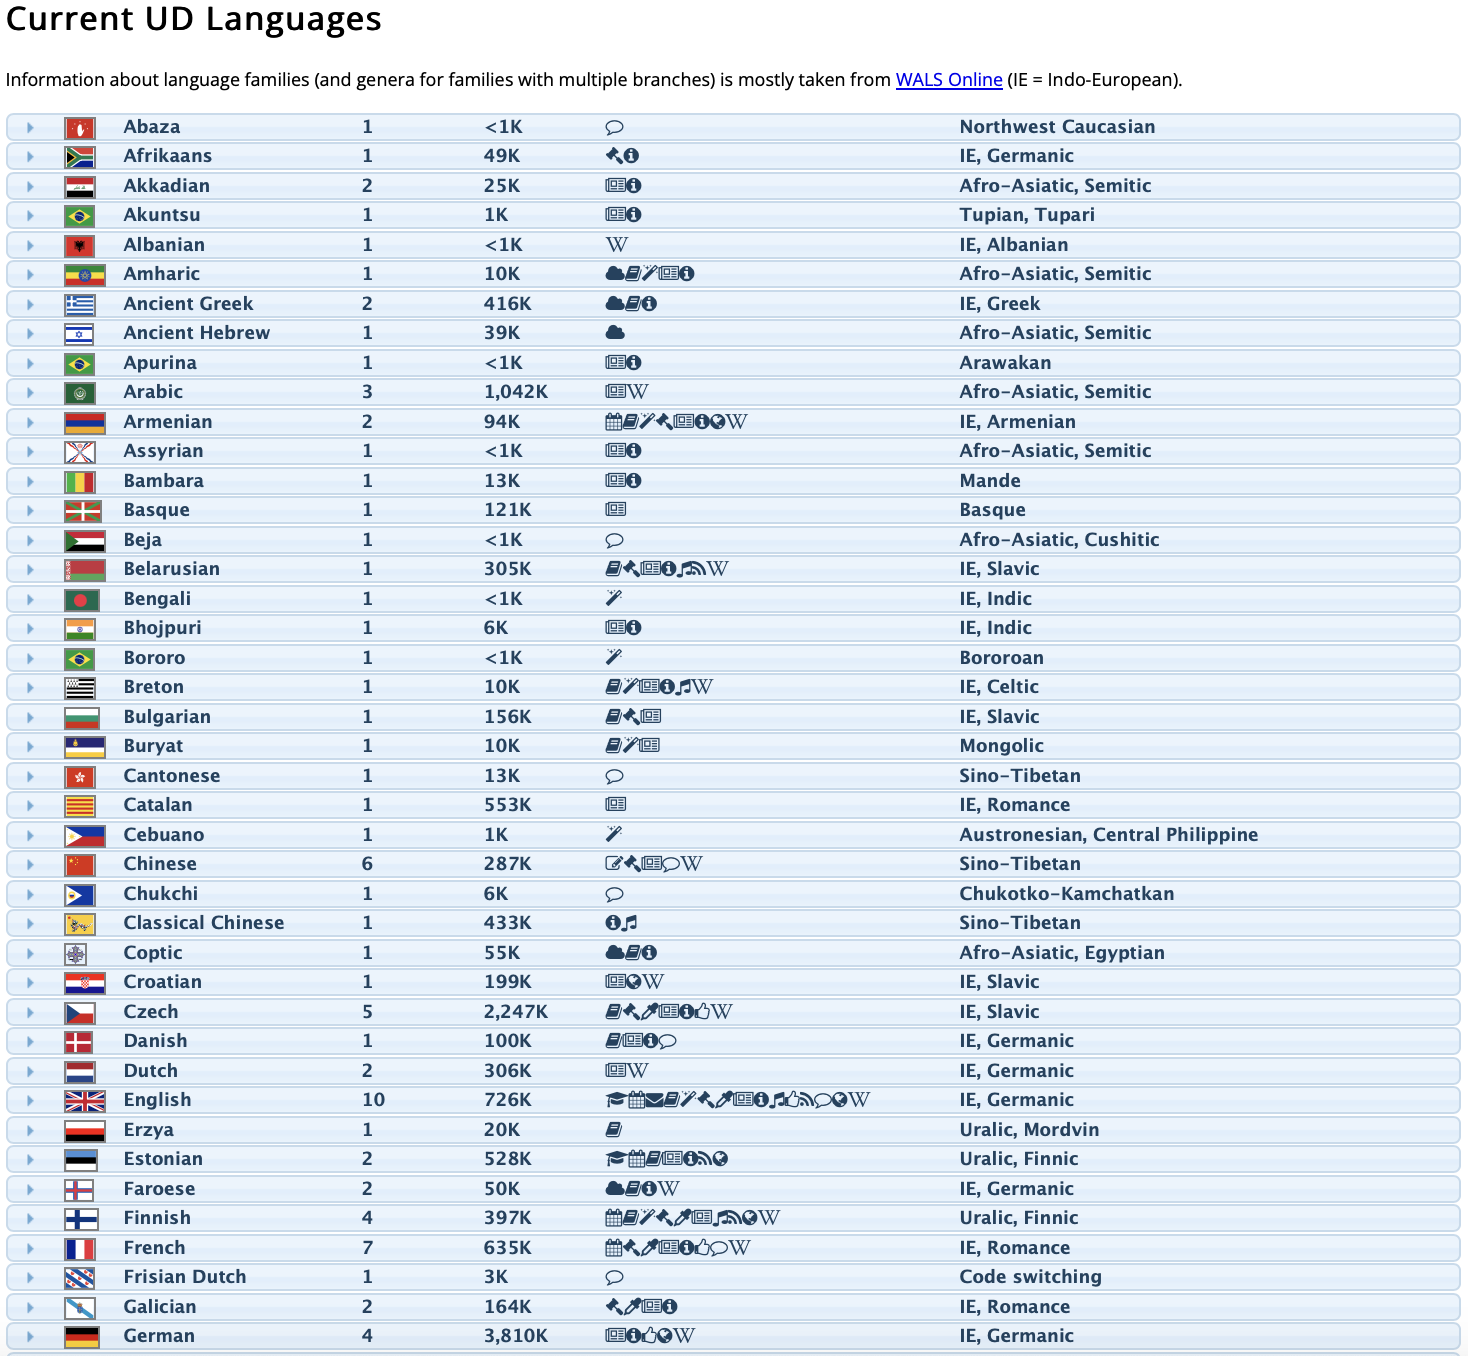
\includegraphics[scale=0.34]{images/UD_Treebank_Listing}
\end{column}%
\end{columns}
\end{frame}

\begin{frame}{The UD Data Repository}
\begin{columns}[T] % align columns
\begin{column}{.51\textwidth}
\centering
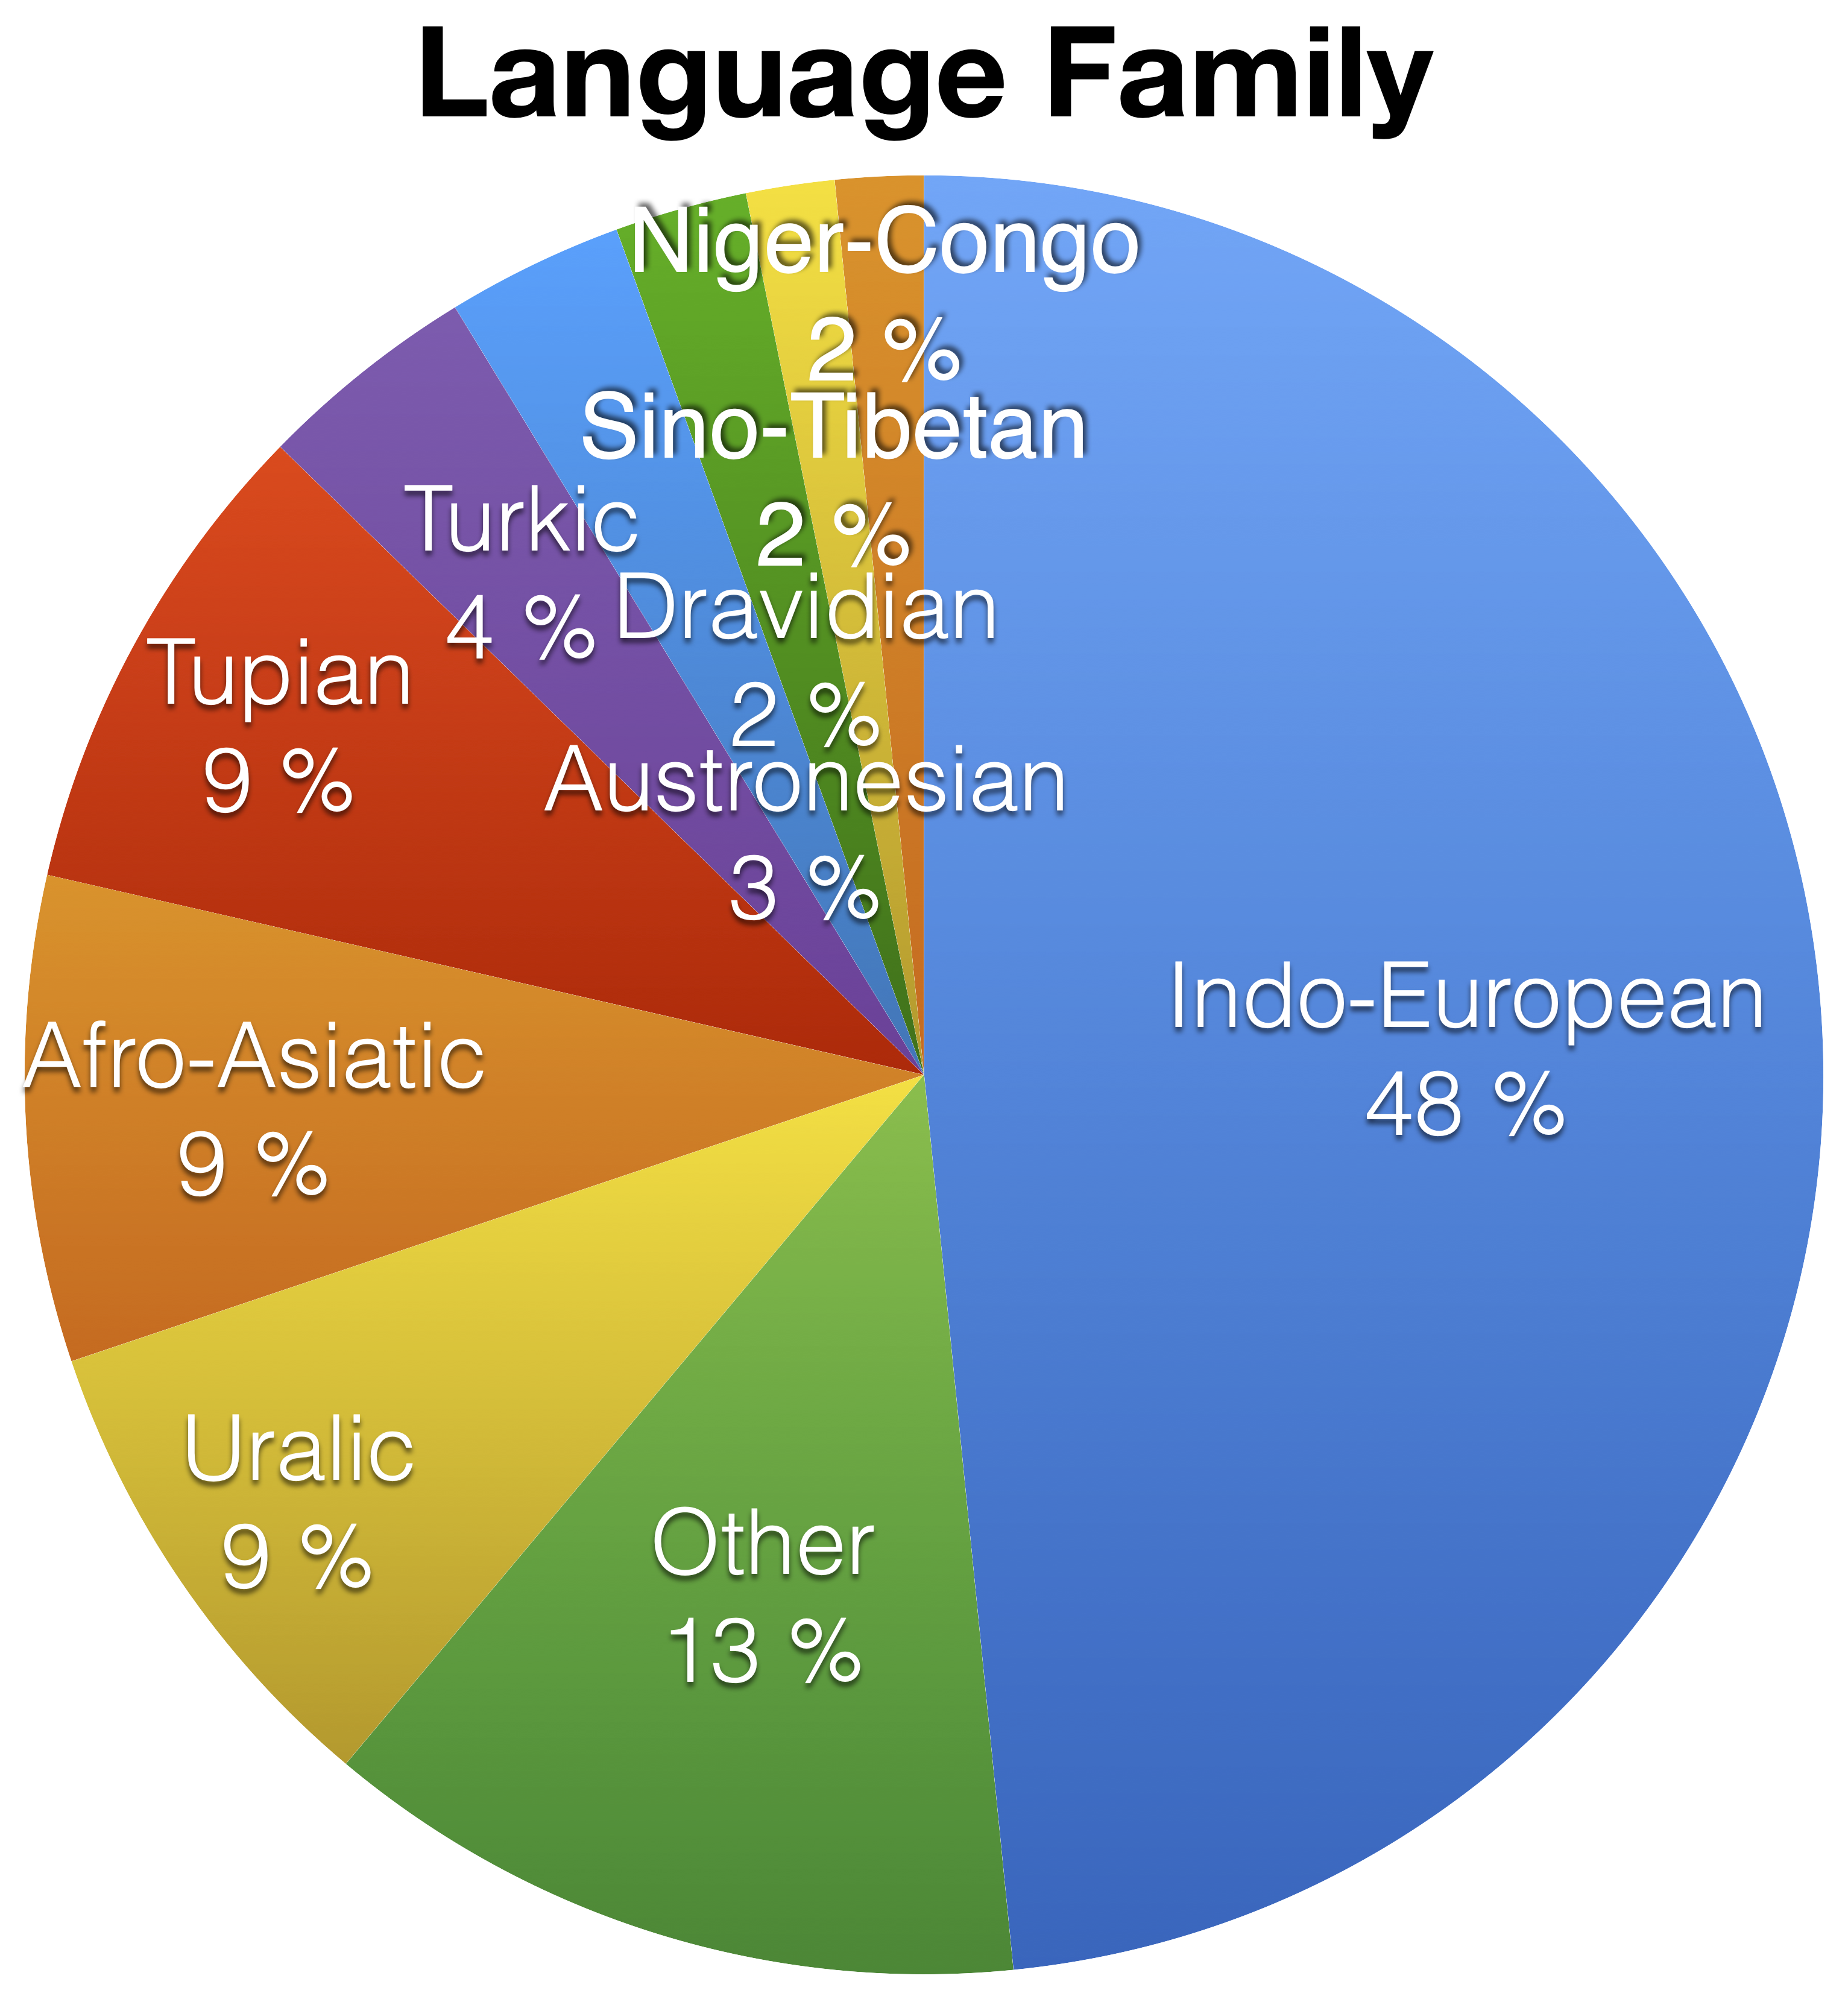
\includegraphics[scale=0.056]{images/LanguageFamily}
\end{column}%
\hfill%
\begin{column}{.49\textwidth}
%\centering
\visible<2>{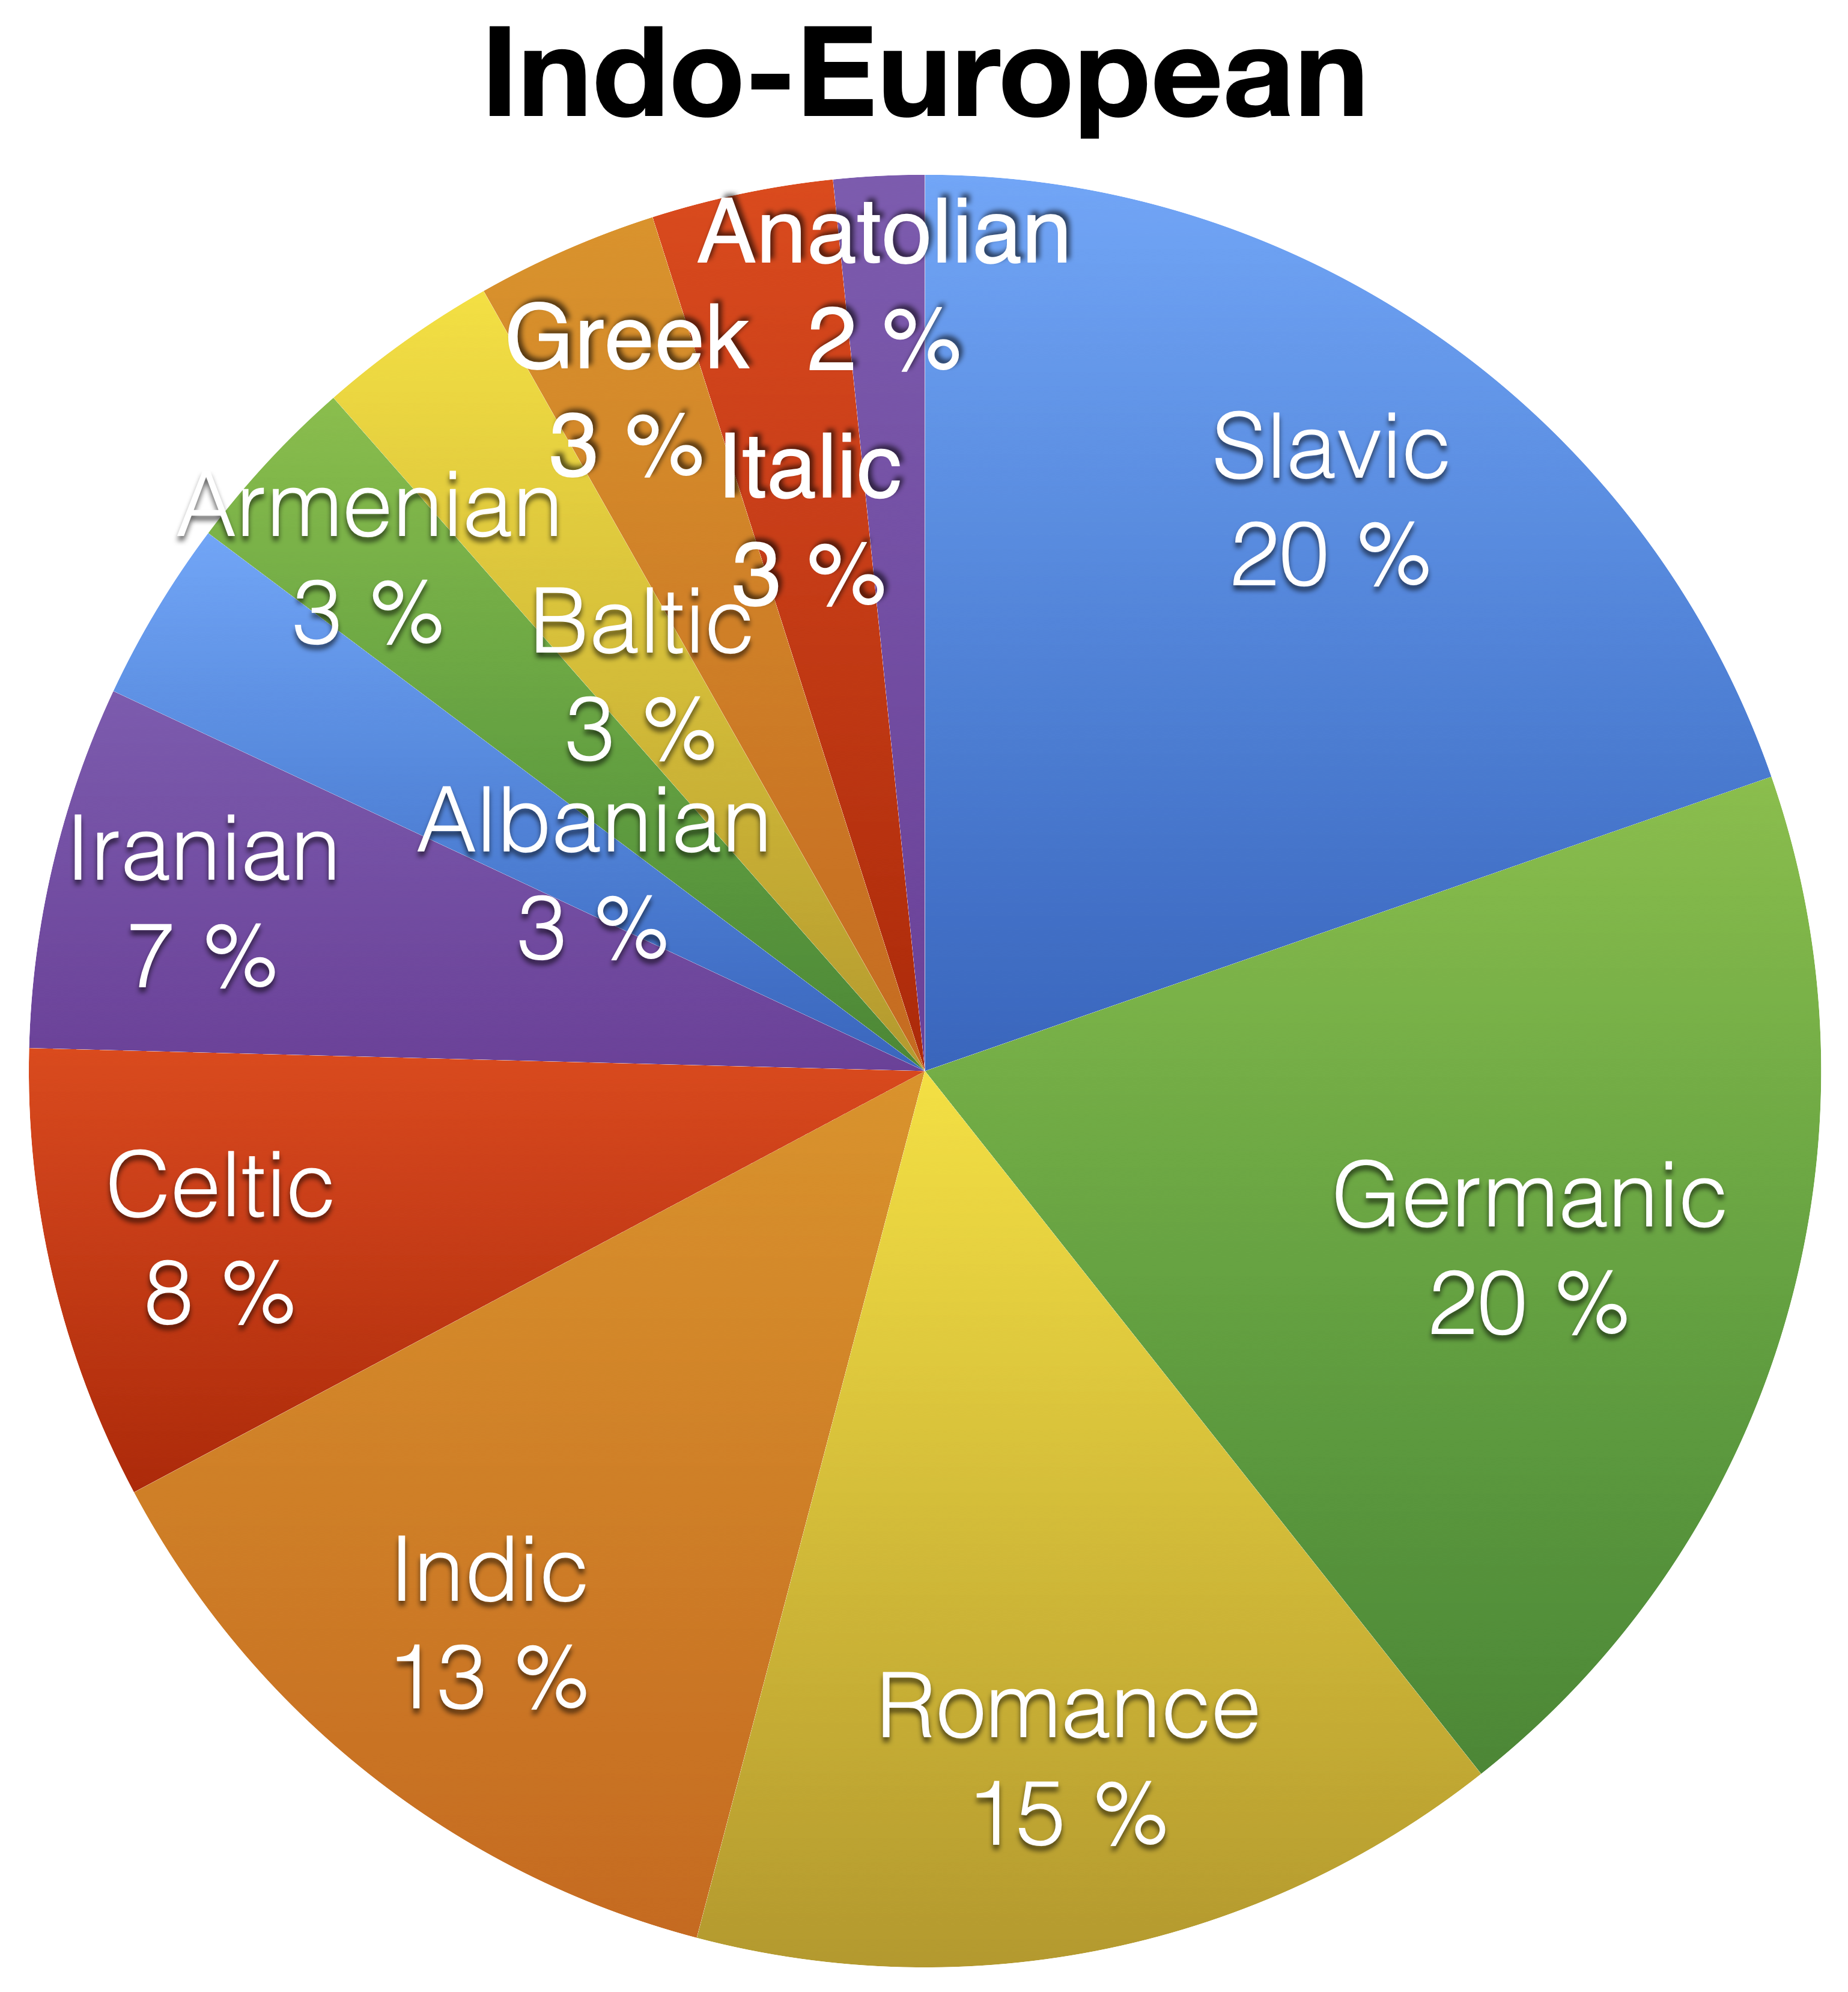
\includegraphics[scale=0.056]{images/IndoEuropean}}
\end{column}%
\end{columns}
\end{frame}

\begin{frame}{The UD Community --- A Big Tent}
\centering
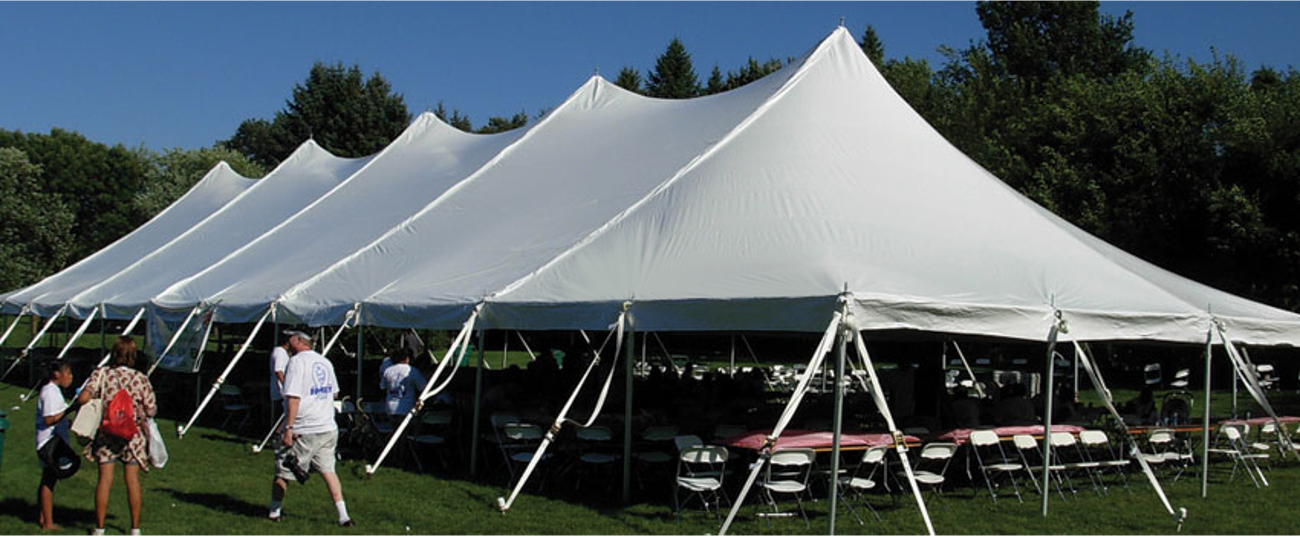
\includegraphics[scale=0.4]{images/BigTent}

\bigskip
\begin{itemize}
\item Universal guidelines group --- universal guidelines, data validation and releases
\item Treebank developers --- treebanks and language-specific documentation 
\item Treebank users --- research in NLP and linguistics based on UD resources
\item Anyone can join!
\end{itemize}
\end{frame}

\begin{frame}{The UD Community --- A Literature Survey}
\centering
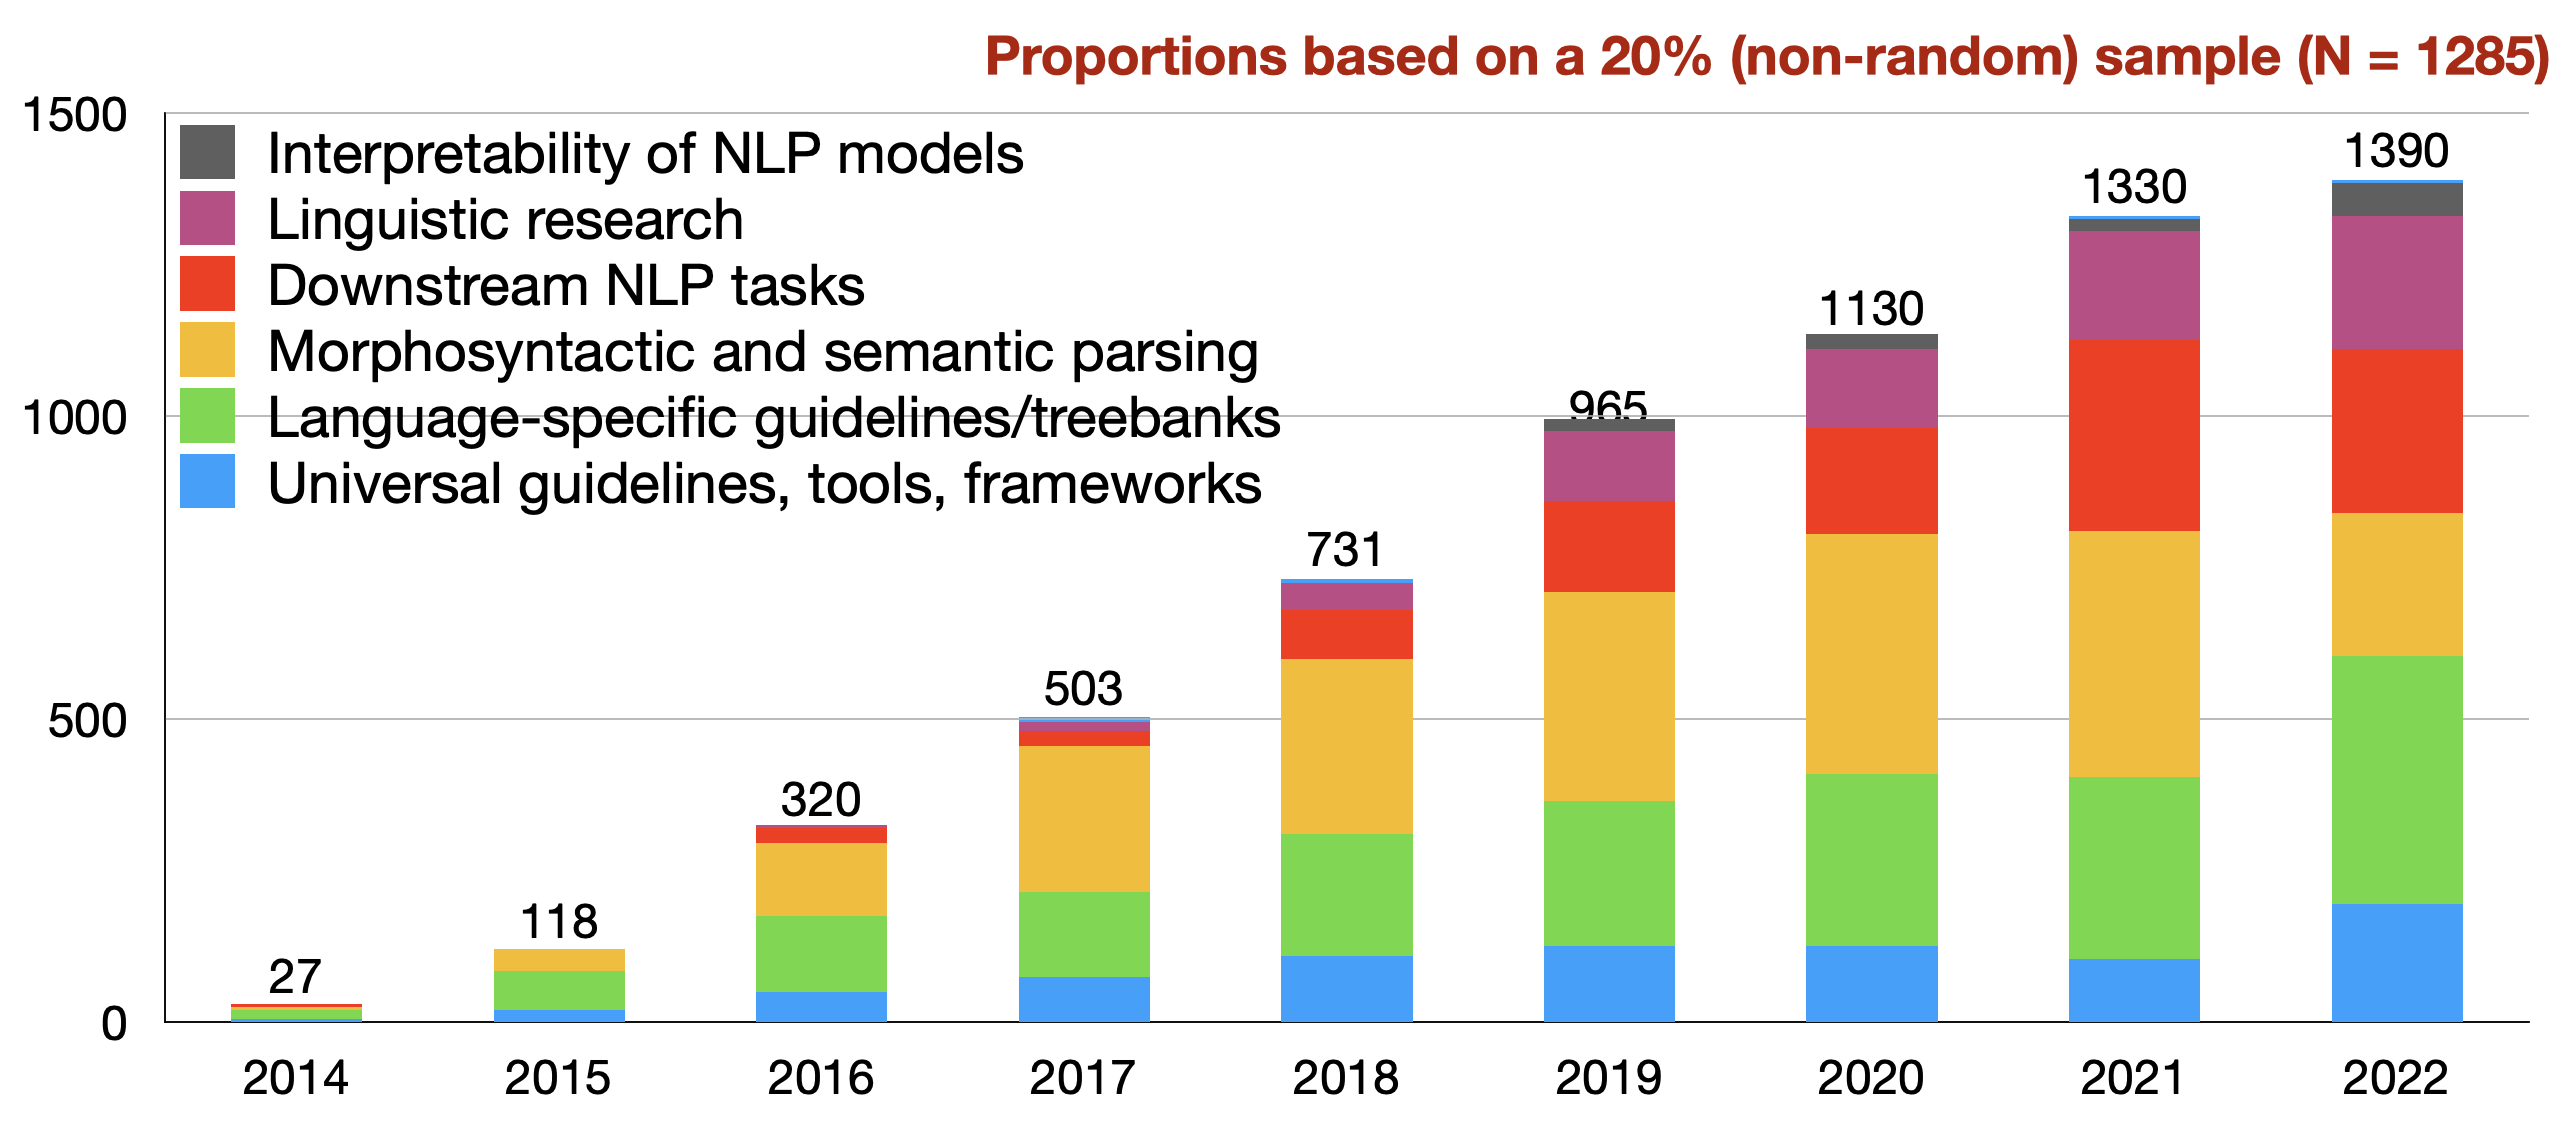
\includegraphics[scale=0.15]{images/LiteratureSurvey}

\bigskip
\begin{itemize}
\item Categories of research in a sample of 277 publications from 2022 (top 20\%):
\begin{itemize}
\item Universal guidelines, tools, frameworks (14\%)
\item Language-specific guidelines/treebanks (30\%)
\item Morphosyntactic and semantic parsing (17\%)
\item Downstream NLP tasks (19\%)
\item Interpretability of NLP models (4\%)
\item Linguistic research (16\%)
\end{itemize}
\end{itemize}
\end{frame}

\begin{frame}{Outline}
\begin{enumerate}
\item Introduction [Joakim]
\item Syntactic annotation [Marie]
\item []~~~~~\textbf{BREAK} [10 min]
\item Word segmentation and morphological annotation [Dan]
\item Annotation exercise [Joakim]
\item []~~~~~\textbf{BREAK} [10 min]
\item Adding a new language to UD [Dan]
\item Questions and discussion [Marie]
\end{enumerate}
\end{frame}

\end{document}

\begin{frame}{Manning's Law}
\hfill
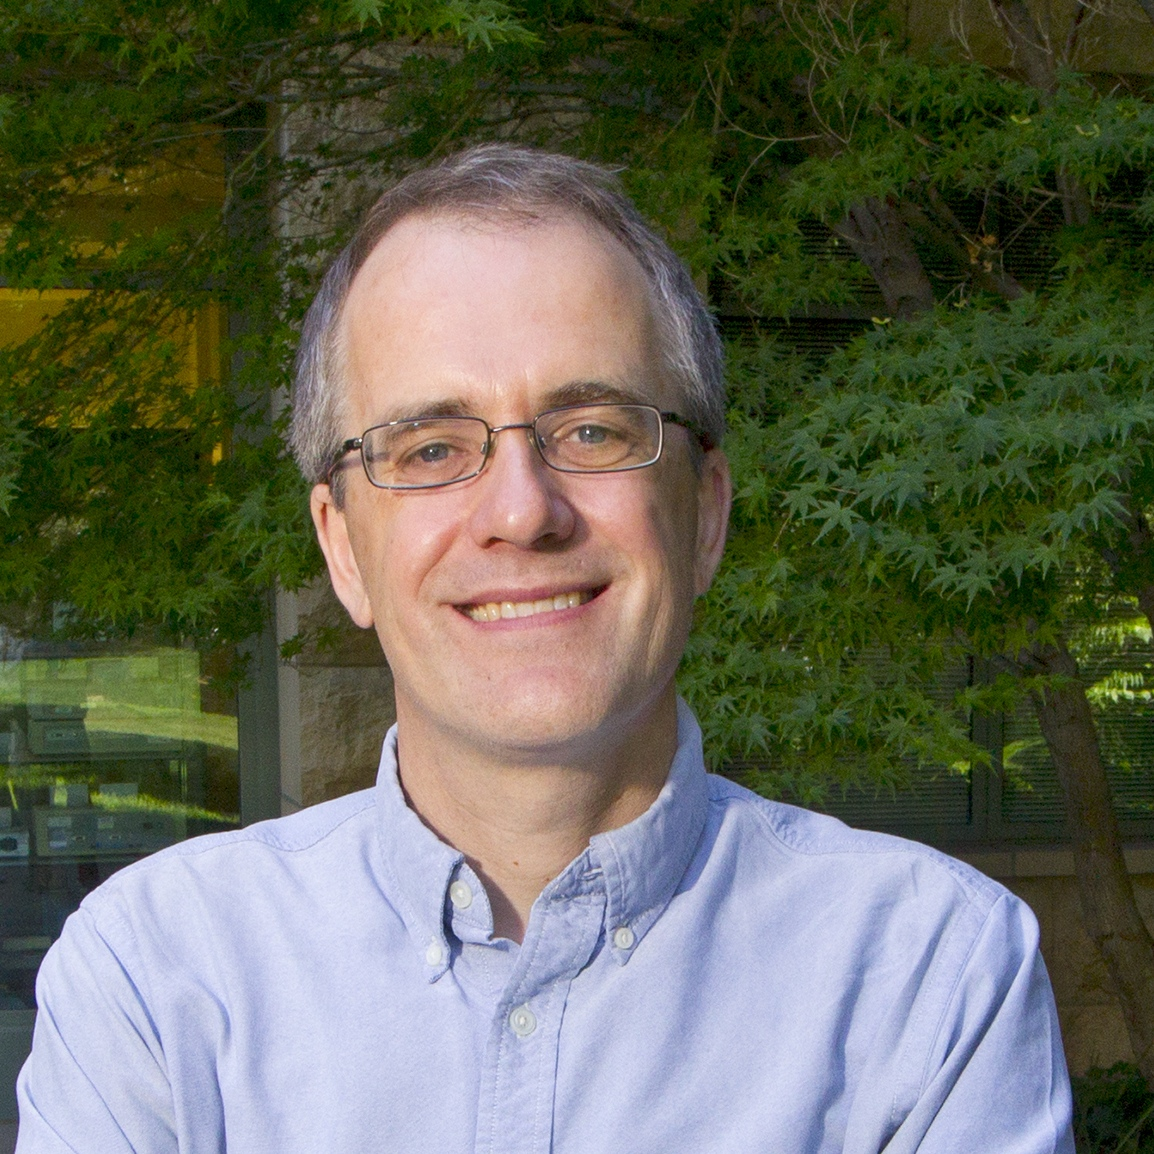
\includegraphics[scale=0.2]{chris}

\noindent
The secret to understanding the design of UD is to realize that it is a very subtle compromise between approximately 6 things:
\begin{enumerate}
\item UD needs to be satisfactory for analysis of individual languages.
\item UD needs to be good for linguistic typology.%, i.e., bring out parallelism across languages and language families.
\item UD must be suitable for rapid, consistent annotation.
\item UD must be suitable for computer parsing with high accuracy.
\item UD must be easily comprehended and used by a non-linguist.%, whether a language learner or an NLP engineer. %We refer to this as seeking a habitable design, and it leads us to favor traditional grammar notions and terminology.
\item UD must provide good support for downstream NLP tasks. % (relation extraction, reading comprehension, machine translation, \ldots).
\end{enumerate}
It’s easy to come up with a proposal that improves UD on one of these dimensions. The interesting and difficult part is to improve UD while remaining sensitive to all these dimensions.
\end{frame}

\begin{frame}{An Open Community Effort}
Join the fun!
\end{frame}


%%%%%%%% Filip's notes from out Hangout on 16.2.

% Enhanced dependencies - where do they go?

% Alan Akbik - PropBanks
% Parallel Treebanks

% Can cut "Extending UD annotation"
%    - hands-on exercises?
%    - find an error maybe? cross-lingual search?
%    - Quiz solvable using search

% 2nd half:
   % tools, hands-on, resources, big parsed data

% Shared Task -> Dan

% Resources and infrastructure
%% what treebanks we have, conllu, github

% Tools
%% search, UDPipe-SyntaxNet, annotation tools (none), udapi?

% Usage of UD
  % - word order
  % Galactic dependencies

%%%%%%%%% End %%%%%%%%%


% 30 mins = 20-30 slides

% Constructions, strategies, representations

%   - Basic clauses (intransitive, transitive, nominal)

%   - Nominal phrases

%   - Complex clauses (coordination, subordination)

%   - Multiword expressions

%   - Ellipsis

\end{document}
